%File: main.tex
\documentclass[letterpaper]{article}
\usepackage{url,graphicx,xcolor}
\usepackage{times}
\usepackage{helvet}
\usepackage{courier}
\usepackage[]{faikrmod3} % without guidelines
\frenchspacing
\setlength{\pdfpagewidth}{8.5in}
\setlength{\pdfpageheight}{11in}

\pdfinfo{
/Title (A Bayesian Network for Predicting Diabetic Patient Readmission via Hill-Climb Structure Learning)
/Author (Kaveh Haji Najaf)}
\setcounter{secnumdepth}{0}
\begin{document}

\title{A Bayesian Network for Predicting Diabetic Patient Readmission via Hill-Climb Structure Learning}
\author{Kaveh Haji Najaf\\
Master's Degree in Artificial Intelligence, University of Bologna\\
kaveh.hajinajaf@studio.unibo.it
}
\maketitle

\begin{abstract}
\begin{quote}
This project models 30-day hospital readmission risk for diabetic patients as a discrete Bayesian Network whose structure is learned from the UCI \emph{Diabetes 130-US Hospitals} dataset with Hill Climb search. We systematically explore the hyperparameter space of the search itself — structure score, maximum in-degree, number of features, category cardinality — with a 24-configuration grid search selected by validation macro-F1, and find that the scoring function and search depth matter far more than any single feature choice. The winning configuration (K2 score, max in-degree 3, 12 features) clearly outperforms a majority-class baseline on held-out test data, reaching a macro-F1 of 0.312 versus 0.248 for the baseline, while remaining compact and interpretable.
\end{quote}
\end{abstract}


\section{Introduction}
\subsection{Domain}
Hospital readmission of diabetic patients is a well-studied problem in clinical informatics: unplanned readmissions are costly and often preventable. We model this domain using the UCI \emph{Diabetes 130-US Hospitals for Years 1999--2008} dataset~\cite{diabetes130}, which records 101{,}766 inpatient encounters across 130 US hospitals, labelled with whether the patient was readmitted within 30 days (\texttt{<30}), after 30 days (\texttt{>30}), or not at all (\texttt{NO}). Prior work on this data~\cite{strack2014impact} used logistic regression; we instead learn the domain structure automatically with a Bayesian Network.

\subsection{Aim}
The purpose of this project is to learn a Bayesian Network structure for the three-class \texttt{readmitted} outcome using Hill Climb search, and — more importantly — to understand \emph{how} the search's own hyperparameters shape the result. Hill Climb is a greedy, score-based procedure, so its outcome depends heavily on choices such as the scoring function and the maximum number of parents allowed per node; rather than picking these by hand, we run a grid search over them and select by validation performance, treating the search configuration itself as the main object of study.

\subsection{Method}
We used the \texttt{pgmpy} library~\cite{pgmpy} throughout. Before any learning, the raw extract was cleaned following \cite{strack2014impact}'s preprocessing (deduplicating patients, excluding hospice/death discharges, grouping diagnosis codes into 9 clinical categories, mapping coded IDs to labels) to obtain a smaller set of clinically meaningful, low-cardinality columns; this is a one-off, data-independent preparation step and not the focus of this report. We then: (i) split the data 64\%/16\%/20\% into train/validation/test, stratified on the target; (ii) ranked candidate features by mutual information with the target, greedily filtering redundant ones (pairwise normalized mutual information $\geq 0.90$); (iii) discretized numeric columns into quantile bins and capped categorical cardinality, mapping rare/unseen values to \texttt{Other}; and (iv) fitted CPDs with Bayesian estimation using a BDeu prior (equivalent sample size 10).

The structure itself is learned by \textbf{Hill Climb search}: starting from an empty graph, it greedily applies the single edge addition, removal, or reversal that most increases a decomposable structure score, subject to acyclicity and a maximum-in-degree bound that caps how many parents (and hence how large the CPT) a node may have, until no local move improves the score further. We compared the \texttt{BIC} and \texttt{K2} scores. Because the outcome of this search is sensitive to the scoring function, the in-degree bound, and the feature set it searches over, we ran an exhaustive \textbf{grid search} over 24 configurations — number of features $\in\{8,12,16\}$, score $\in\{$BIC, K2$\}$, max in-degree $\in\{2,3\}$, category cap $\in\{8,12\}$, at a fixed 4 numeric bins — training a candidate network for each and selecting by validation macro-F1 (log-loss as tie-breaker).

\subsection{Results}
The grid search shows the search configuration matters more than any individual feature: every \texttt{BIC}-scored candidate converged to the same macro-F1 of 0.330 regardless of the in-degree bound or category cap, whereas \texttt{K2} improved from 0.339 (max in-degree 2) to 0.351 (max in-degree 3), and adding features beyond 12 gave no further gain. The winning configuration (12 features, K2, max in-degree 3, category cap 8) was retrained on train+validation and reaches a held-out test macro-F1 of 0.312 (accuracy 0.604), versus 0.248 (accuracy 0.593) for a majority-class baseline.

\section{Model}

\begin{figure}[t]
    \centering
    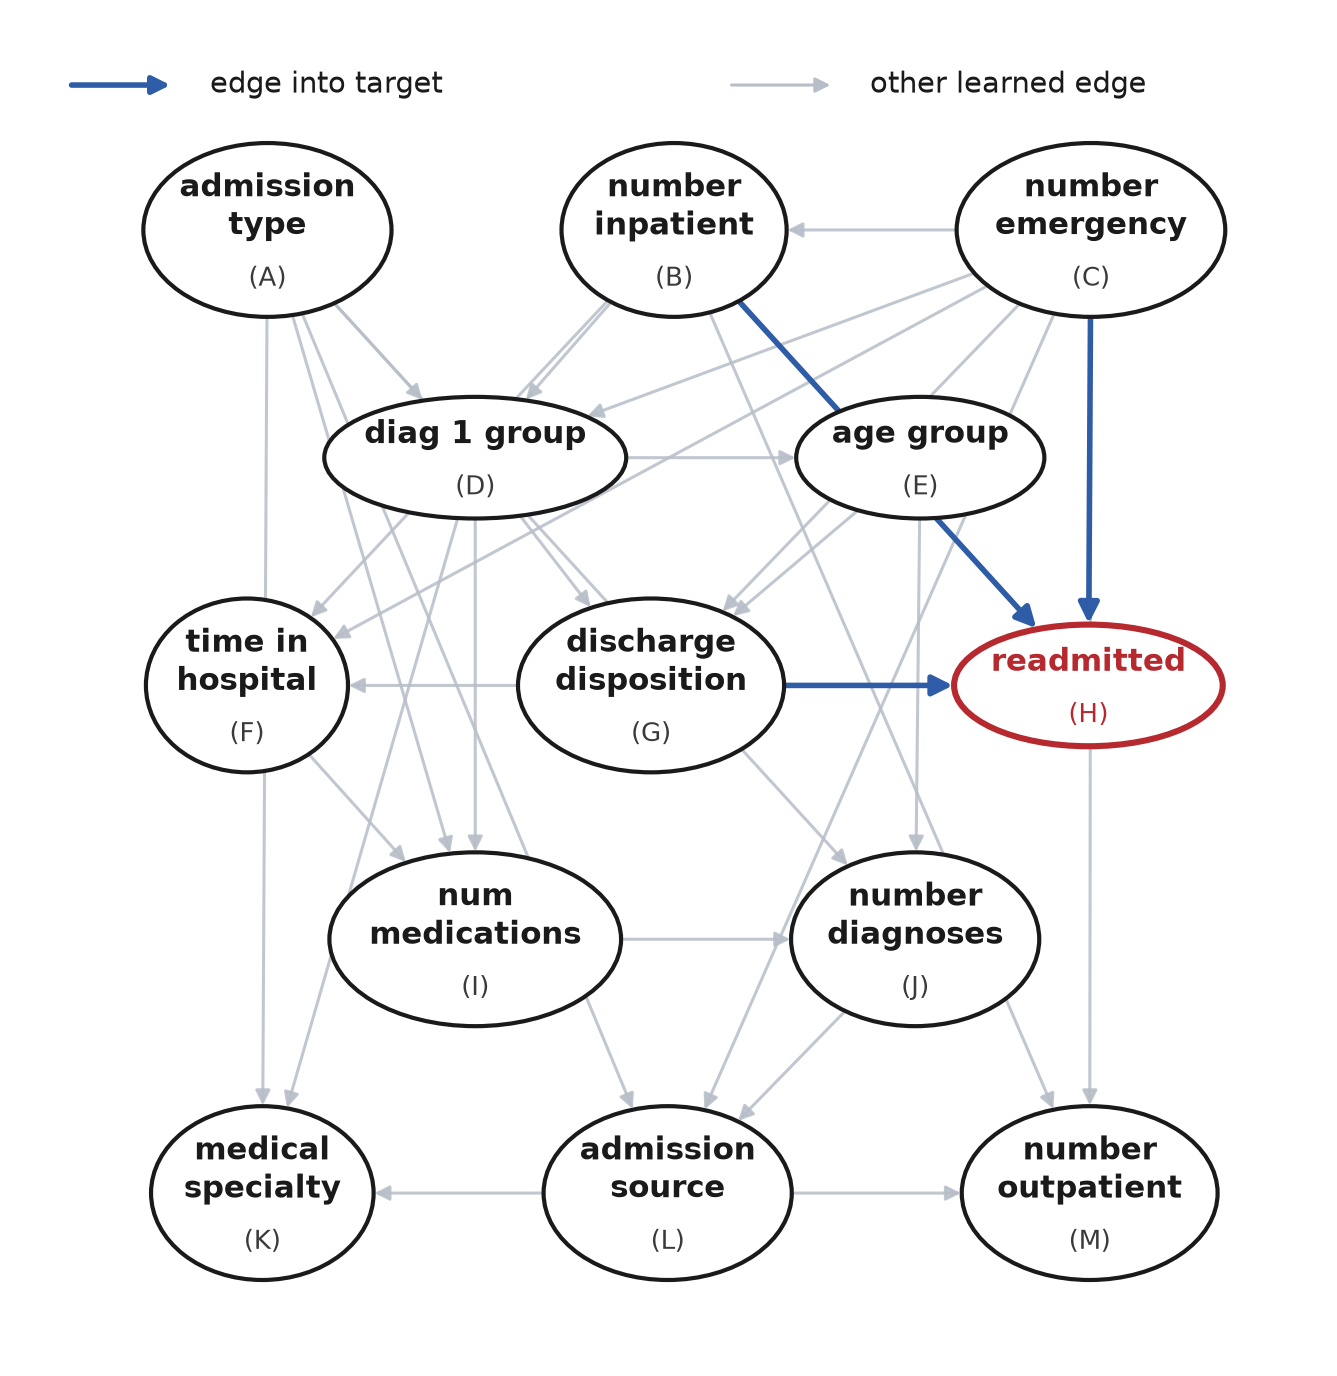
\includegraphics[width=\columnwidth]{figures/bn_structure.png}
    \caption{Structure learned by Hill Climb search (K2 score, max in-degree 3) over the 12 selected features, drawn as a hierarchical DAG with sources at the top and sinks at the bottom; edges into the target are highlighted in blue. \texttt{readmitted} is the red target node.}
    \label{fig:network}
\end{figure}

The network (Figure~\ref{fig:network}) has 12 feature nodes plus the target \texttt{readmitted}, connected by 29 directed edges. The nodes are: \texttt{number\_inpatient}, \texttt{number\_outpatient} and \texttt{number\_emergency} (utilization counts in the prior year), \texttt{discharge\_disposition}, \texttt{admission\_type} and \texttt{admission\_source} (categorical encounter metadata), \texttt{time\_in\_hospital}, \texttt{num\_medications} and \texttt{number\_diagnoses} (numeric, quantile-binned into 4 states), \texttt{medical\_specialty} and \texttt{age\_group} (categorical, capped to the 8 most frequent values plus \texttt{Other}/\texttt{Missing}), and \texttt{diag\_1\_group}, the primary diagnosis grouped into 9 clinical categories. \texttt{readmitted} itself has three states (\texttt{<30}, \texttt{>30}, \texttt{NO}) and, as learned by Hill Climb, has three direct parents — \texttt{number\_inpatient}, \texttt{number\_emergency} and \texttt{discharge\_disposition} — meaning the other 9 selected features influence the target only indirectly, through the surrounding graph.

No part of the structure or CPDs was manually specified: the DAG in Figure~\ref{fig:network} is exactly what Hill Climb search returned for the winning grid-search configuration, and the CPDs are BDeu-smoothed estimates fitted afterwards.

\section{Analysis}

\subsection{Experimental setup}
We evaluated the final network, retrained on the combined training and validation splits, on the untouched 20\% test split (13{,}998 encounters), against a majority-class \texttt{DummyClassifier} baseline trained on the same data. We report accuracy, balanced accuracy, macro/weighted F1, log-loss, macro ROC-AUC/PR-AUC, and the multiclass Brier score. Since the three classes are strongly imbalanced (roughly 59\%/32\%/9\% for \texttt{NO}/\texttt{>30}/\texttt{<30}), we treat macro-F1, not accuracy, as the primary metric, as a trivial majority-class predictor already reaches 59\% accuracy. Given the grid-search results, we expected the K2-scored, deeper-search network to beat the baseline by a moderate margin, struggling most on the minority \texttt{<30} class — the hardest and clinically most actionable class to predict.

\subsection{Results}
On the test split, the network reaches accuracy 0.604, balanced accuracy 0.358 and macro-F1 0.312, versus 0.593, 0.333 and 0.248 for the majority baseline — a clear, if modest, improvement, consistent with the validation-time gain the grid search predicted for this configuration over shallower or BIC-scored alternatives. Per-class $F_1$ is 0.75 for \texttt{NO}, 0.16 for \texttt{>30} and only 0.02 for \texttt{<30} (recall 0.01): the model recognizes non-readmitted patients far better than the rare \texttt{<30} class, which the confusion matrix confirms is almost always predicted as \texttt{NO} — unsurprising given how small and diffuse that class is (9\% of test encounters) relative to the max-in-degree cap and discretization granularity the search was constrained to. As a secondary sanity check, the cleaning stage's output (69{,}987 encounters) closely matches the 69{,}984 reported by \cite{strack2014impact}, giving confidence that any remaining error comes from the modelling choices analyzed above rather than a faulty pipeline.

\section{Conclusion}
Treating Hill Climb's own hyperparameters as the primary object of study, rather than fixing them by hand, was informative: the scoring function dominated the outcome (K2 consistently beat BIC, which collapsed to the same structure regardless of the in-degree bound), a deeper in-degree bound further helped K2, and feature count saturated quickly. The resulting network is compact and interpretable and still clearly beats a majority-class baseline, though the gain is concentrated in the majority class and the model struggles with early (\texttt{<30}) readmissions. A natural extension would be to grid-search a class-weighted or two-stage objective directly, rather than macro-F1 alone, to see whether the minority class benefits from the same kind of systematic search.


\section{Links to external resources}


\bigskip

\bibliographystyle{aaai}
\bibliography{faikrmod3}


\end{document}
